% This file was converted to LaTeX by Writer2LaTeX ver. 1.2
% see http://writer2latex.sourceforge.net for more info
\documentclass{article}
\usepackage[ascii]{inputenc}
\usepackage[T1]{fontenc}
\usepackage[english]{babel}
\usepackage{amsmath}
\usepackage{amssymb,amsfonts,textcomp}
\usepackage{array}
\usepackage{hhline}
\usepackage{graphicx}
\title{}
\begin{document}
Importarea si exportarea datelor


\bigskip

Programarea sistemului central de import/export care sa permita introducerea

automata a datelor, atat cele de suport cat si datele sociale


\bigskip

Importer-ul proceseaza si salveaza in baza de date fisiere XML ce corespund standardului DDI-Codebook (Data Documentation Initiative, http://www.ddialliance.org/Specification/DDI-Codebook/


\bigskip

Se foloseste un pachet de clase Java derivat de catre JAXB pornind de la definitia in format 'XML Schema' a DDI-Codebook; acest pachet se numeste 'ro.roda.ddi'.

Este posibil sa se salveze si din formatul DDI nativ direct in baza de date (practic se parseaza si se construiesc la runtime tabelele corespunzand tag-urilor din formatul DDI).


\bigskip

Cele mai importante tag-uri din fisierele DDI ce sunt procesate sunt:


\bigskip

[docDscr] - Document description

Aceasta sectiune trebuie sa fie cat mai completa posibil, si cuprinde informatii despre

autor, persoane si organizatii responsabile de continut si drepturile de proprietate intelectuala, producatorul, sursa fisierului (codebook-ul original).


\bigskip

[stdyDscr] -{}- Study description

informatii despre colectia de date, studiu, sau compilatie pe care o descrie documentatia DDI;

informatii despre cum ar trebui citat studiul, cine a colectat, corectat, agregat datele, cine distribuie datele, cuvinte-cheie despre continutul datelor, un rezumat al continutului datelor, metode de colectare si procesare a datelor etc.


\bigskip

[fileDscr] -{}- File Description

informatii despre fisierele cu date care formeaza o colectie; aceasta sectiune poate fi repetata pentru colectii cu fisiere multiple.

Aici se pot face si referinte la {\textquotedbl}summary data description{\textquotedbl} si la aspecte de metodologie anterior descrise, care se aplica unor anumite fisiere din colectie.


\bigskip

[dataDscr] -{}- Data description

descrierea variabilelor (si optional a unor calcule statistice pe baza valorilor acestora).


\bigskip

[otherMat] -{}- Other Materials

permite includerea si etichetarea altor materiale care sunt in legatura cu studiul;

sectiunea poate servi si ca un {\textquotedbl}container{\textquotedbl} pentru alte materiale in format electronic (de ex. chestionare, note de codificare, SPSS/SAS/Stata fisiere de setup si altele, manuale pentru utilizatori, ghiduri pentru continuarea cercetarii, glosare, instructiuni pentru operatori, harti, scheme de baze de date, dictionare de date, informatii despre valorile-lipsa etc.).


\bigskip

Impreuna cu sistemul de import al datelor si metadatelor, RODA va stoca si fisierele originale. In anumite situatii, fisierele originale vor fi importate treptat printr-un proces asistat de catre operatori. Pentru aceasta, este nevoie de un sistem de tip content repository care sa permita intretinerea fisierelor statice, impreuna cu versiunile acestora si orice alte informatii conexe disponibile. Un astfel de sistem a fost implementat folosind componentul Apache Jackrabbit care este o implementare a API{}-ului Java Content Repository (JCR -- specificat in cadrul normelor JSR 170 si 283. O descriere a acestui sistem se poate gasi in ANEXA 1. 


\bigskip

Sistemul de executie automata a actiunilor (cron)


\bigskip

Programarea sistemului de executie asincrona a operatiilor de intretinere

impreuna cu componentul dedicat al interfetei de administrare.


\bigskip

Sistemul CRON pentru RODA se bazeaza pe componentul TaskScheduler din Spring 3.0, component care ofera o varietate de metode pentru rularea unei operatii la un anumit moment programat in viitor. 


\bigskip

In jurul acestui sistem, echipa RODA a construit un sistem de stocare a informatiilor cu privire la aceste operatii si a rezultatelor executiilor acestora, precum si o interfata grafica utilizata pentru programarea actiunilor asincrone si pentru urmarirea rezultatelor acestora. In figura urmatoare se poate vedea principalul ecran al acesteia. In anexa 1 sunt disponibile detalii si toate ecranele interfetei.


\bigskip

  [Warning: Image ignored] % Unhandled or unsupported graphics:
%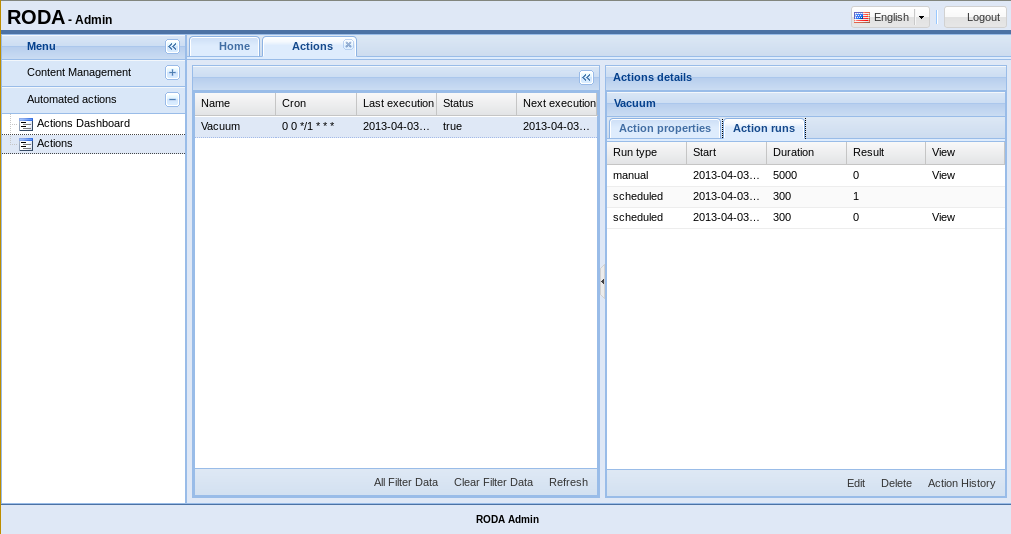
\includegraphics[width=6.5in,height=3.4307in]{RezumatRODAfaza5-img/RezumatRODAfaza5-img001.png}
 

Jurnalizare


\bigskip

Programarea sistemului de inregistrare si recuperare a tuturor modificarilor

bazei de date si datelor asociate.


\bigskip

Sistemul utilizat in aplicatia informatica RODA este Hibernate Envers. Alegerea acestui sistem pentru asigurarea auditului se bazeaza, in primul rand, pe faptul ca aplicatia utilizeaza tehnologia Hibernate pentru maparea nivelului obiectual al aplicatiei in baza de date relationala. Hibernate furnizeaza biblioteca Envers, acum parte a nucleului sau, ce permite integrarea functionalitatii de jurnalizare (audit).


\bigskip

Tabelele de audit ale RODA se afla intr-o schema a bazei de date (audit), separata de schema in care se afla tabelele corespunzatoare entitatilor modelului.


\bigskip

Fiecare tabel de audit contine cateva coloane specifice:

\begin{itemize}
\item id -- cheia primara a entitatii originale (poate contine mai multe \ \ coloane, in cazul cheilor primare compuse)
\item revision \ number -- un numar intreg, ce reprezinta numarul reviziei din tabelul de \ \ revizii
\item revision type -- un numar intreg reprezentand tipul reviziei
\item coloanele auditate din tabelul original.
\end{itemize}

\bigskip

Cheia primara a tabelului de audit este compusa din cheia primara a entitatii originale si numarul reviziei; poate exista cel mult o inregistrare de audit pentru o instanta de entitate data la o anumita revizie.

Entitatea curenta este stocata atat in tabelul original, cat si in cel de audit. Astfel, sistemul de interogare furnizat de aceasta solutie de audit este foarte puternic. O linie din tabelul de audit, avand cheia primara id, revizia n si valoarea unui camp v are urmatoarea semnificatie: entitatea al carei cod este id are valoarea v pentru campul specificat incepand de la revizia n. Astfel, daca dorim sa gasim o entitate la revizia m, trebuie sa cautam linia din tabelul de audit al carei numar al reviziei cel mai apropiat numar mai mic sau egal decat m. Daca nu este gasita o astfel de linie, sau daca este gasita o linie marcata deleted, atunci entitatea nu exista la revizia respectiva.
\end{document}
